\chapter{Pravděpodobnostní modely časových řad}

\section{Stochastické procesy}

Stochastický proces lze obecně popsat jako ``statistický fenomén, který se vyvíjí v čase podle určitých zákonů pravděpodobnosti". Matematicky pak lze stochastický proces definovat soubor náhodných pozorování, která jsou uspořádaná v čase, přičemž tato pozorování mohou být jako spojitá tak diskrétní. Spojitou náhodnou veličinu v čase $t$ označujeme jako $X(t)$ a diskrétní pak jako $X_t$.

Na pozorované hodnoty lze nahlížet jako na jednu konkrétní realizaci časové řady z množiny všech možných pozorování. Tuto množinu nazýváme souborem (ensemble). Každý člen tohoto souboru je pak realizací stochastického procesu.

Jedním ze způsobů, jak popsat časovou řadu, je specifikovat sdruženou pravděpodobnostní funkci $X(t), ..., X(t_n)$ pro libovolnou množinu časů $t_1, ..., t_n$ a libovolnou hodnotu $n$. Tato možnost je však spíše hypotetická. Nejčastěji se časová řada popisuje pomocí tzv. momentů, zejména pak prvního a druhého momentu, které jsou známé jako střední hodnota a rozptyl popř. autokovariance.

Střední hodnota časové řady $\mu(t)$ je definována jako
\begin{equation}
\mu(t) = E[X(t)],
\end{equation}
rozptyl $\sigma^2(t)$ jako
\begin{equation}
\sigma^2(t) = Var[X(t)]
\end{equation}
a konečně autokovariance mezi $X(t_1)$ a $X(t_2)$ jako
\begin{equation}
\gamma(t_1, t_2) = E\{[X(t_1) - \mu(t)][X(t_2) - \mu(t_2)]\}.
\end{equation}

\section{Stacionární procesy}

Časová řada je striktně stacionární, pokud je její sdružená pravděpodobnostní funkce pro $X(t_1), ..., X(t_n)$ shodná se sdruženou pravděpodobnostní funkcí pro $X(t_1 + \tau), ..., X(t_n + \tau)$ pro všechna $t_1, ..., t_n, \tau$.

Pokud je $n = 1$, striktní stacionarity implikuje shodné pravděpodobností rozdělení náhodné veličiny $X(t)$ pro všechna $t$ za předpokladu, že $\mu(t) = \mu$ a $\sigma^2(t) = \sigma^2$, kde $\mu$ a $\sigma^2$ jsou konečné.

Pro $n = 2$ striktní stacionarita vyžaduje, aby sdružená pravděpodobnostní funkce pro $X(t_1)$ a $X(t_2)$ závisela pouze na $(t_2 - t_1)$, tj. tzv zpoždění. Autokovarianční funkce $\gamma(t_1, t_2)$ taktéž závisí pouze na $(t_2 - t_1)$, tj. můžeme ji vyjádřit jako
\begin{equation}
\gamma(\tau) = E\{[X(t) - \mu][X(t+\tau) - \mu]\} = Cov[X(t), X(t + \tau)].
\end{equation}
Standardizovaná autokovarianční funkce se pak nazývá autokorelační funkcí a je definována jako
\begin{equation}
\rho(\tau) = \frac{\gamma(\tau)}{\gamma(0)}
\end{equation}
a měří korelaci mezi $X(t)$ a $X(t + \tau)$.

\subsection{Stacionarity druhého stupně}

V praxi často vhodné definovat stacionaritu méně restriktivně než je tomu ve výše uvedeném textu. Proces nazýváme stacionárním druhého řádu (second-order stationary) nebo také slabě stacionárním (weakly stationary), pokud je jeho střední hodnota konstantní a jeho autokorelační funkce závisí pouze na zpoždění $\tau$, tj. pokud platí
\begin{equation}
E[X(t)] = \mu
\end{equation}
a
\begin{equation}
cov[X(t), X(t + \tau)] = \gamma(\tau).
\end{equation}
Připomeňme, že pro $\tau = 0$ odpovídá autokovarianční funkce rozptylu. Dále musí platit, že jak střední hodnota tak rozptyl musí být konečné. Tato definice stacionarity bude používána v následujícím textu.

\section{Autokorelační funkce}

Předpokládejme, že stacionární stochastický proces $X(t)$ má střední hodnotu $\mu$, rozptyl $\sigma^2$ a autokovarianční funkci $\gamma(\tau)$. Autokorelační funkce je pak definována jako
\begin{equation}
\rho(\tau) = \frac{\gamma(\tau)}{\gamma(0)} = \frac{\gamma(\tau)}{\sigma^2}.
\end{equation}
Připomeňme, že $\rho(0) = 1$.

Autokorelační funkce je sudou funkcí zpoždění $\tau$, tj.
\begin{equation}
\rho(\tau) = \rho(-\tau).
\end{equation}
Tato vlastnost říká, že korelace mezi $X(t)$ a $X(t + \tau)$ je stejná jako mezi $X(t)$ a $X(t - \tau)$.

Pro autokorelační funkci dále platí $|\rho(\tau) \le 1|$, což je standardní vlastnost korelace.

Ačkoliv lze daný stochastický proces charakterizovat jedinečnou kovarianční strukturou, opačné tvrzení není pravdivé. Jinými slovy, je možné nalézt několik rozdílných stochastických procesů, které mají shodnou autokorelační funkci.

\section{Několik užitečných stochastických procesů}

\subsection{Čistě náhodný proces}
Diskrétní proces nazýváme čistě náhodným procesem, pokud se skládá z posloupnosti náhodných veličin $\{Z_t\}$, které jsou vzájemně nezávislé a sledují stejné pravděpodobnostní rozdělení. Z této definice vyplývá, že tento proces má konstantní střední hodnotu a rozptyl a že
\begin{equation}
\gamma(k) = Cov(Z_t, Z_{t + k}) = 0, ~~~ k = \pm 1, \pm 2, ...
\end{equation}
Protože střední hodnota a autokovariance nejsou funkcí času, jedná se o slabě stacionární proces. Ve skutečnosti je také zřejmé, že se jedná také o striktně stacionární proces. Autokorelační funkce čistě náhodného procesu je definována jako
\begin{equation}
\rho(k) =
\begin{cases}
\begin{split}
1 & \quad k = 0\\
0 & \quad k = \pm 1, \pm 2, ...
\end{split}
\end{cases}
\end{equation}
Čistě náhodnému procesu se někdy také říká bílý šum (white noise) a to zejména v inženýrské terminologii. Procesy tohoto typu jsou užitečné v mnoha situacích, zejména jako stavební bloky složitějších procesů jako jsou např. modely klouzavého průměru, které si představíme v následujících kapitolách.

\subsection{Náhodná procházka}

Předpokládejme, že $\{Z_t\}$ je diskrétní čistě náhodný proces se střední hodnotou $\mu$ a rozptylem $\sigma^2_Z$. Proces $\{X_t\}$ je nazýván náhodnou procházkou, pokud
\begin{equation}
X_t = X_{t - 1} + Z_t.
\end{equation}
Tento proces obvykle ``začíná" v čase $t = 0$, což implikuje
\begin{equation}
X_1 = Z_1
\end{equation}
a
\begin{equation}
X_t = \sum_{i = 1}^t Z_i.
\end{equation}
Lze snadno dokázat, že $E(X_t) = t \mu$ a $Var(X_t) = t \sigma^2_Z$. Protože se střední hodnota i rozptyl mění s časem $t$, je náhodná procházka nestacionárním procesem. Nicméně první diference náhodné procházky
\begin{equation}
\nabla X_t = X_t - X_{t - 1} = Z_t
\end{equation}
je čistě náhodný proces a tím pádem stacionární.

Jedním z nejznámějších příkladů časových řad, které se chovají jako náhodná procházka, je denní vývoj cen akcií.

\subsection{Proces klouzavého průměru}

Předpokládejme, že $\{Z_t\}$ je čistě náhodný proces s nulovou střední hodnotou a rozptylem $\sigma^2_Z$. Proces $\{X_t\}$ je procesem klouzavého průměru (moving average proces) řádu $q$, zkráceně označovaného jako $MA(q)$, pokud
\begin{equation}
X_t = \beta_0 Z_t + \beta_1 Z_{t - 1} + ... + \beta_q Z_{t - q},
\end{equation}
kde $\{\beta_i\}$ jsou konstanty, kde typicky $\beta_0 = 1$.

Z výše uvedené definice je zřejmé
\begin{equation}
E(X_t) = 0
\end{equation}
a
\begin{equation}
Var(X_t) = \sigma^2_Z \sum_{i = 0}^q \beta_i^2,
\end{equation}
protože jednotlivá $Z$ jsou nezávislá. Dále platí
\begin{equation}
\begin{split}
\gamma(k) & = Cov(X_t, X_{t + k})\\
 & = Cov(\beta_0 Z_t + ... + \beta_q Z_{t - q}, \beta_0 Z_{t + k} + ... + \beta_q Z_{t + k - q})\\
 & =
 \begin{cases}
 0 & \quad k > q\\
 \sigma^2_Z \sum_{i = 0}^{q - k} \beta_i \beta_{i + k} & \quad k = 0, 1, ..., q\\
 \gamma(-k) & \quad k < 0
 \end{cases}
\end{split}
\end{equation}
protože
\begin{equation}
Cov(Z_s, Z_t) = 
\begin{cases}
\sigma^2_z & \quad s = t\\
0 & \quad s \ne t
\end{cases}
\end{equation}

Vzhledem k tomu, že $\gamma(k)$  nezávisí na $t$ a střední hodnota procesu je konstantní, je proces klouzavého průměru slabě stacionární pro všechny hodnoty $\{\beta_i\}$. Navíc, protože jednotlivá $Z$ sledují normální rozdělení, sledují normální rozdělení také jednotlivá $X$, což má za následek striktně stacionární normální proces.

Autokorelační funkce procesu klouzavého průměru řádu $q$ je dána
\begin{equation}
\rho(k) =
\begin{cases}
1 & \quad k = 0\\
\frac{\sum_{i = 0}^{q-k} \beta_i \beta_{i + k}}{\sum_{i = 0}^q \beta_i^2} & \quad k = 1, ..., q\\
0 & \quad k > q\\
\rho(-k) & \quad k < 0
\end{cases}
\end{equation}
Za pozornost stojí skutečnost, že pro časové posuny vyšší než $q$ nabývá autokorelační funkce hodnoty nula, což je specifická vlastnost $MA(q)$ procesu.

Ačkoliv není třeba na $\{\beta_i\}$ klást žádné požadavky, aby byl $MA(q)$ stacionárním procesem, je žádoucí stanovit hodnoty $\{\beta_i\}$ tak, aby byl $MA(q)$ proces tzv. invertibilním. Pro ilustraci uvažujme dva$MA(1)$ procesy
\begin{equation}
(A) \quad X_t = Z_t + \theta Z_{t - 1}
\end{equation}
a
\begin{equation}
(B) \quad X_t = Z_t + \frac{1}{\theta}Z_{t - 1}.
\end{equation}
Lze snadno dokázat, že tyto dva rozdílné $MA(1)$ procesy mají shodnou autokorelační funkci. Jinými slovy, autokorelační funkce nepředstavuje jedinečnou identifikaci MA procesu. Jestliže pomocí opakované substituce vyjádříme oba dva výše uvedené procesy pomocí $X_t, X_{t - 1}, ...$, získáme
\begin{equation}
(A) \quad Z_t = X_t - \theta X_{t-1} + \theta^2 X_{t-2} - ...
\end{equation}
a
\begin{equation}
(B) \quad Z_t = X_t - \frac{1}{\theta}X_{t - 1} + \frac{1}{\theta^2}X_{t - 2} - ...
\end{equation}
Jestliže $|\theta| < 1$, pak řada A konverguje, kdežto řada B nikoliv. Proto odhad založený na reziduích povede přirozeně k řadě A. Proto, je-li $|\theta| < 1$, je řada A tzv. invertibilní, kdežto řada B nikoliv. Podmínka invertibility tak zajišťuje jedinečný MA proces pro každou autokorelační funkci.

Podmínku invertibility obecného $MA(q)$ procesu lze nejsnadněji vyjádřit pomocí operátoru $B$, který je definován jako
\begin{equation}
B^j X_t = X_{t - j} \quad \textit{pro všechna} ~ j.
\end{equation}
Rovnici (3.16) tak můžeme vyjádřit ve tvaru
\begin{equation}
X_t = (\beta_0 + \beta_1 B + ... \beta_q B^q)Z_t = \theta(B)Z_t.
\end{equation}
Proces $MA(q)$ je invertibilní, pokud se kořeny rovnice (s ohledem k $B$ jako ke komplexní proměnné a nikoliv jako k operátoru)
\begin{equation}
\theta(B) = \beta_0 + \beta_1 B + ... + \beta_q B^q = 0
\end{equation}
nacházejí mimo jednotkový kruh. Např. pro $MA(1)$ má tato rovnice tvar $\theta(B) = 1 + \theta B$ s kořenem $B = -\frac{1}{\theta}$. Kořen je tak mimo jednotkový kruh, pokud $|\theta| < 1$.

Na pravou stranu rovnice (3.16) lze přidat libovolnou konstantu, typicky střední hodnotu $\mu$. Tímto způsobem docílíme toho, že $E(X_t) = \mu$ bez toho, abychom ovlivnili autokorelační funkci.

\subsection{Autoregresní proces}

Předpokládejme, že $\{Z_t\}$ je čistě náhodný proces s nulovou střední hodnotou a rozptylem $\sigma^2_Z$. Proces $\{X_t\}$ je procesem autoregresním procesem (autoregressive proces) řádu $p$, pokud
\begin{equation}
X_t = \alpha_1 X_{t - 1} + ... + \alpha_p X_{t - p} + Z_t.
\end{equation}
V následujícím textu budeme autoregresní proces řádu $q$ označovat jako $AR(q)$.

\subsubsection{AR(1)}

Při zkoumání vlastností autoregresního procesu začněme autoregresním modelem řádu jedna, tj.
\begin{equation}
X_t = \alpha X_{t-1} + Z_t.
\end{equation}
Proces $AR(1)$ je taktéž někdy nazýván Markovovým procesem. Postupnou substitucí můžeme výše uvedenou rovnici vyjádřit ve tvaru
\begin{equation}
X_t = \alpha(\alpha X_{t - 2} + Z_{t - 1}) + Z_t = \alpha^2 (\alpha X_{t - 3} + Z_{t - 2}) + \alpha Z_{t - 1} + Z_t,
\end{equation}
kdy jsme $X_t$ schopni vyjádřit jako nekonečný MA proces
\begin{equation}
X_t = Z_t + \alpha Z_{t - 1} + \alpha^2 Z_{t - 2} + ...
\end{equation}

Rovnici (3.30) je možné vyjádřit také pomocí operátoru $B$ jako
\begin{equation}
(1 - \alpha B)X_t = Z_t,
\end{equation}
takže ve spojení s (3.32) platí
\begin{equation}
X_t = \frac{Z_t}{1 - \alpha B} = (1 + \alpha B + \alpha^2 \beta^2 + ...) Z_t = Z_t + \alpha Z_{t - 1} + \alpha^2 Z_{t - 2} + ...
\end{equation}
Z toho vztahu pak vyplývá
\begin{equation}
E(X_t) = 0
\end{equation}
a
\begin{equation}
Var(X_t) = \sigma_Z^2 (1 + \alpha^2 + \alpha^4 + ...).
\end{equation}
Rozptyl $AR(1)$ procesu je tak konečný, pokud $|\alpha| < 2$, kde
\begin{equation}
Var(X_t) = \frac{\sigma_Z^2}{1 - \alpha^2}.
\end{equation}
Autokovariační funkce je pak definována jako
\begin{multline}
\gamma(k) = E[X_t X_{t + k}] =\\
E\Big[\Big(\sum_i \alpha^i Z_{t-i}\Big)\Big(\sum_j \alpha^j Z_{t+k-j}\Big)\Big] =\\
\sigma_Z^2 \sum_{i=0}^{\infty} \alpha^i \alpha^{k + i} \quad k \ge 0
\end{multline}
a pro $|\alpha| < 1$ konverguje k
\begin{equation}
\gamma(k) = \sigma_Z^2 \sum_{i=0}^{\infty} \alpha^i \alpha^{k + i} = \sigma_Z^2 \sigma_{i = 0} \alpha^{k + 2i} = \sigma_Z^2 \frac{\alpha^k}{1 - \alpha^2} = \alpha^k \sigma_X^2.
\end{equation}
Lze dokázat, že pro $k < 0$ platí $\gamma(k) = \gamma(-k)$. Protože $\gamma(k)$ nezávisí na $t$, je $AR(1)$ slabě stacionární, pokud $|\alpha| < 1$.

Autokorelační funkce je pak dána
\begin{equation}
\rho(k) = \alpha^k \quad k = 0, 1, 2, ...
\end{equation}
Abychom získali sudou funkci definovanou pro všechna celá čísla $k$, můžeme autokorelační funkci vyjádřit jako
\begin{equation}
\rho(k) = \alpha^{|k|} \quad k = 0, \pm 1, \pm 2, ...
\end{equation}

Autokorelační funkci lze také jednoduše získat tak, že budeme a priori předpokládat, že proces je stacionární, implikuje $E(X_t) = 0$. Vynásobme rovnici (3.30) pomocí $X_{t - k}$ a na výsledný vztah aplikujme střední hodnotu. Zjistíme, že pro $k > 0$ za předpokladu $E(Z_t X_{t - k}) = 0$ platí
\begin{equation}
\gamma(-k) = \alpha \gamma(-k + 1).
\end{equation}
Protože $\gamma(k)$ je sudá funkce, musí také platit
\begin{equation}
\gamma(k) = \alpha \gamma(k - 1) \quad k > 0.
\end{equation}
Protože $\gamma(0) = \sigma_X^2$, získáváme $\gamma(k) = \alpha^k \sigma_X^2$ pro $k \ge 0$. Proto platí $\rho(k) = \alpha^k$ pro $k \ge 0$. Protože z definice korelace vyplývá $|\rho(k)| \le 1$, musí platit $|\alpha| \le 1$. Nicméně pokud $|\alpha| = 1$, pak $|\rho(k)| = 1$ pro všechna $k$, což je degenerativní proces. Proto pro stacionární proces musí platit $|\alpha| < 1$.

\begin{figure}[htp]
\centering
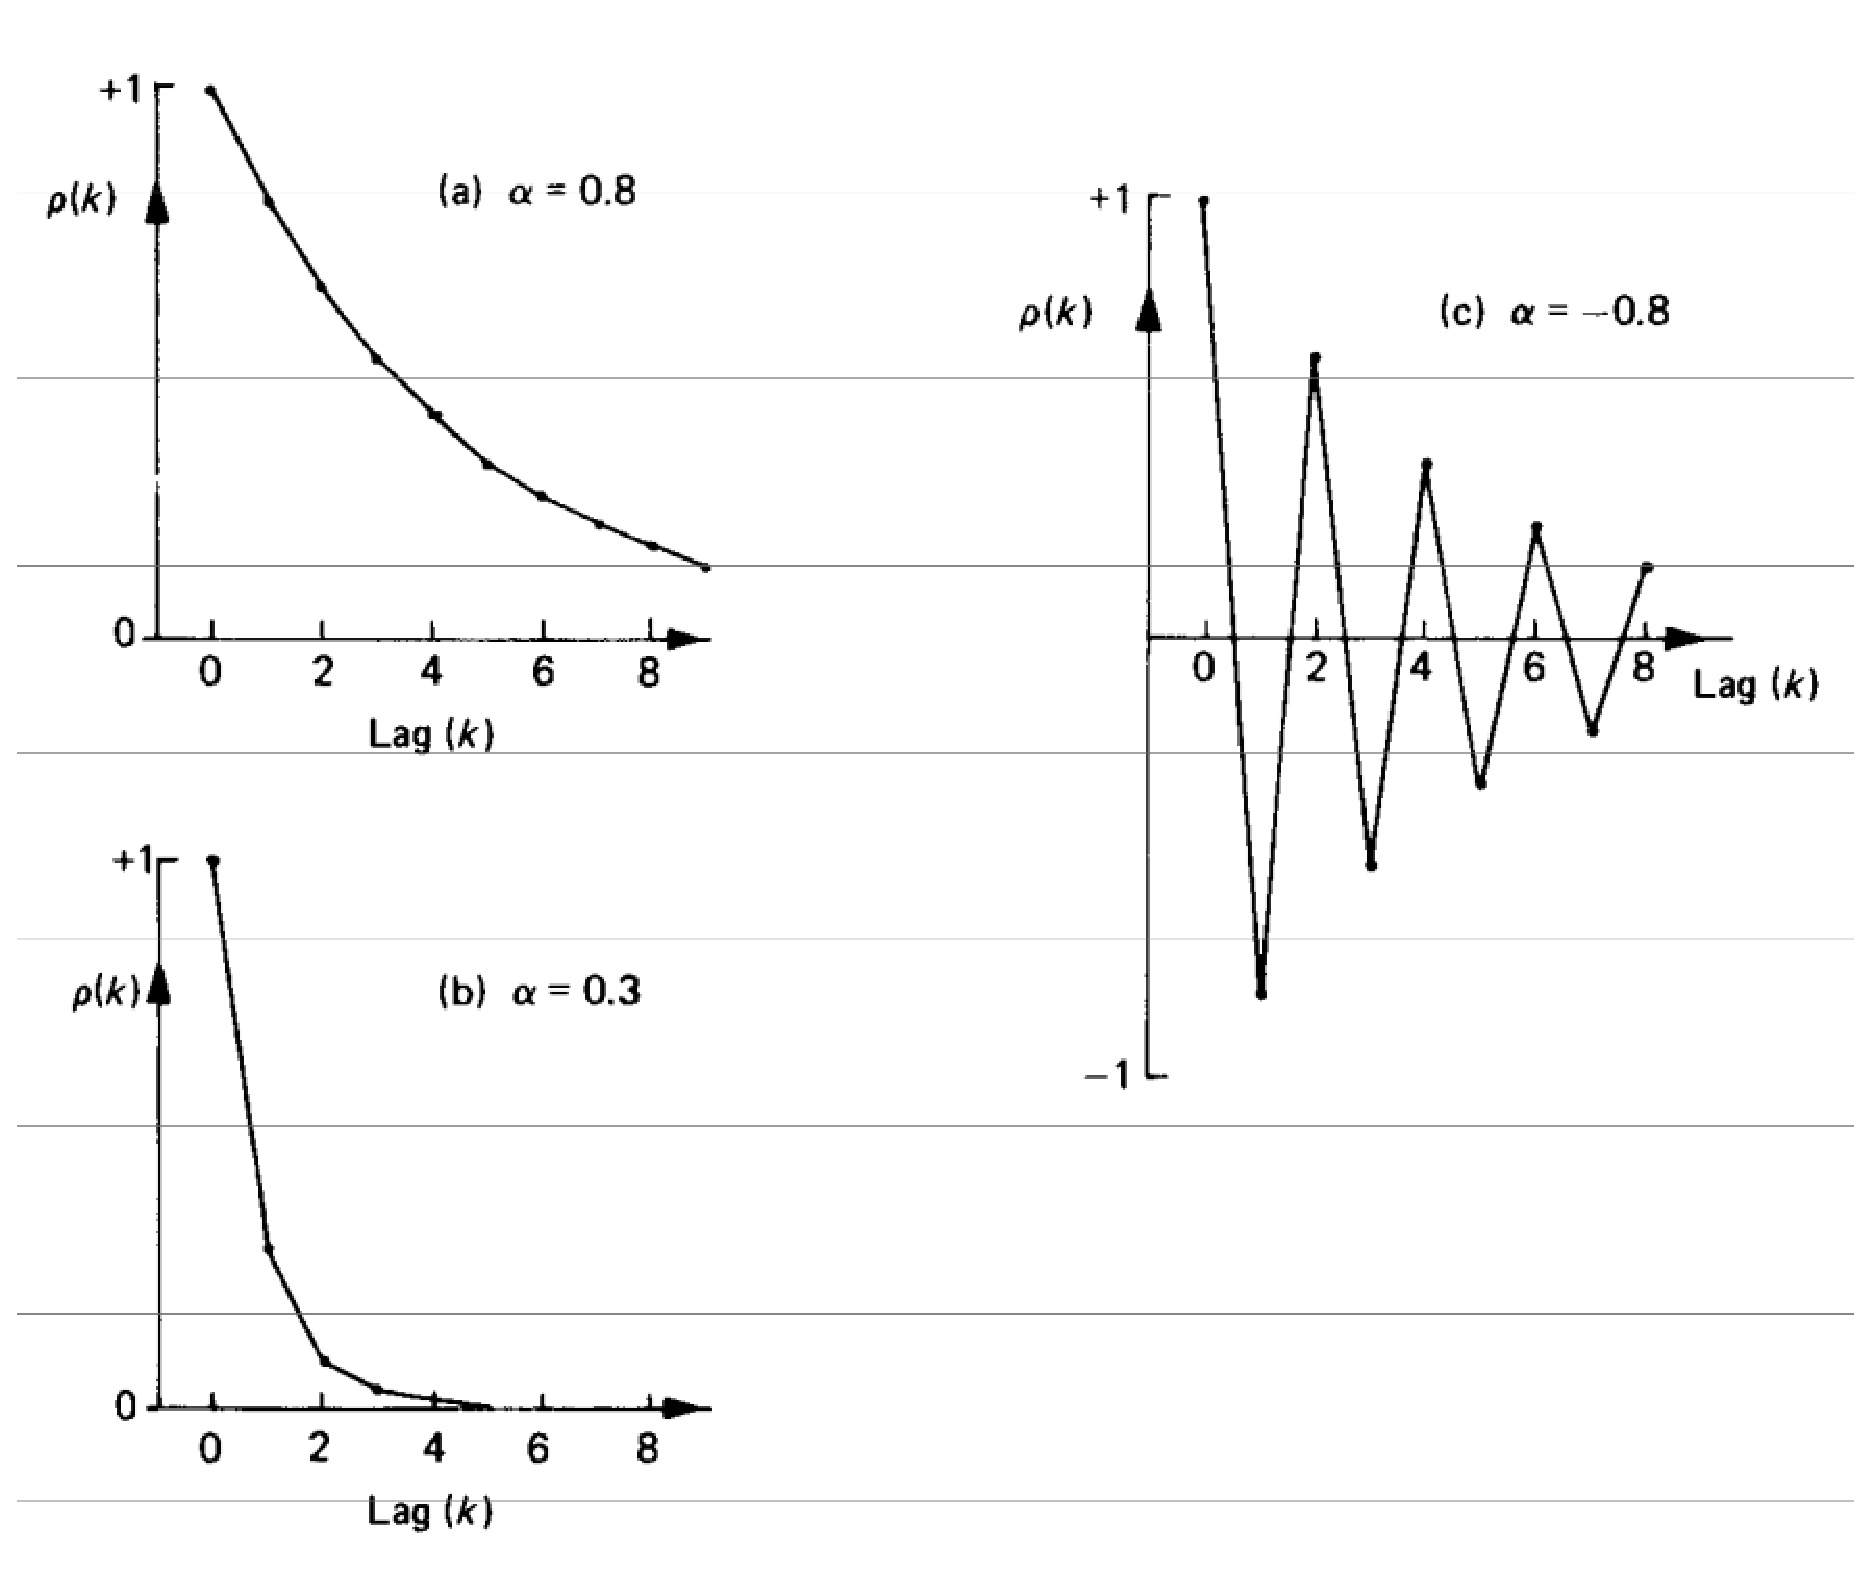
\includegraphics[scale = 0.40]{pictures/figure_3_1.eps}
\caption{Příklady $AR(1)$: (a) $\alpha = 0.8$, (b) $\alpha = 0.3$ a (c) $\alpha = -0.8$}
\label{figure_3_1}
\end{figure}

\subsubsection{AR(q)}

Stejně jako v případě $AR(1)$ i $AR(q)$ jsme schopni vyjádřit jako nekonečný MA proces. Toho lze dosáhnout pomocí postupné substituce nebo pomocí operátoru $B$. Rovnici (3.29) tak lze zapsat jako
\begin{equation}
(1 - \alpha_1 B - ... - \alpha_p B^p)X_t = Z_t
\end{equation}
neboli
\begin{equation}
X_t = \frac{Z_t}{1 - \alpha_1 B - ... - \alpha_p B^p} = f(B)Z_t,
\end{equation}
kde
\begin{equation}
f(B) = \frac{1}{1 - \alpha_1 B - ... - \alpha_p B^p} = 1 + \beta_1 B + \beta_2 B^2 + ...
\end{equation}
Vztah mezi $\{\alpha_i \}$ a $\{\beta_i \}$ lze nalézt pomocí substituce do (3.29) s cílem vyjádřit tento vztah ve tvaru $X_t = f(B)Z_t$. Pokud vyjádříme $X_t$ jako nekonečný MA proces, zjistíme, že $E(X_t) = 0$ a $Var(X_t) = \sigma_Z^2 \sum_i \beta_i^2$. Proces je tedy stacionární, pokud $\sum_i \beta_i^2$ konverguje.

Autokovarianční funkce je dána
\begin{equation}
\gamma(k) = \sigma_Z^2 \sum_{i = 0}^{\infty} \beta_i \beta_{i + k},
\end{equation}
kde $\beta_0 = 1$. Dostatečnou podmínkou pro konvergenci autokovarianční funkce (a tím pádem také stacionarity) je, že $\sum_i |\beta_i|$ konverguje.

Pomocí výše uvedeného postupu je možné odvodit také autokorelační funkci obecného AR procesu, nicméně získání $\{\beta_i\}$ může být poměrně komplikované. Alternativně můžeme předpokládat stacionaritu AR procesu, vynásobit (3.29) členem $X_{t - k}$, aplikovat střední hodnotu na obě strany vzniklé rovnice a následně vydělit $\sigma_X^2$.\footnote{Předpoklad stacionarity nám garantuje, že $\sigma^2_X$ je konečné.} S využitím skutečnosti $\rho(k) = \rho(-k)$ pro všechna $k$ získáme
\begin{equation}
\rho(k) = \alpha_1 \rho(k - 1) + ... + \alpha_p \rho(k - p) \quad k > 0.
\end{equation}
Výše uvedená rovnice se nazývá Yule-Walkerovou rovnicí a má obecné řešení ve tvaru
\begin{equation}
\rho(k) = A_1 \pi_1^{|k|} + ... + A_p \pi_p^{|k|},
\end{equation}
kde $\{\pi_i\}$ jsou kořeny tzv. pomocné rovnice
\begin{equation}
y^p - \alpha_1 y^{p - 1} ... - \alpha_p = 0.
\end{equation}
Konstanty $\{A_i\}$ jsou zvoleny tak, aby byla splněny počáteční podmínky, které se odvíjí od $\rho(0) = 1$, což implikuje $\sum_i A_i = 1$. Prvních $(p - 1)$ Yule-Walkerových rovnic představuje dalších $(p - 1)$ omezení pro $\{A_i\}$ s využitím $\rho(0) = 1$ a $\rho(k) = \rho(-k)$. Z (3.49) je zřejmé, že $\rho(k)$ konverguje k nule s rostoucím $k$, pokud $|\pi_i| < 1$ pro všechna $i$, což je nezbytná a postačující podmínka pro stacionaritu procesu.

Ekvivalentním způsobem vyjádření podmínky stacionarity je, že kořeny rovnice
\begin{equation}
\phi(B) = 1 - \alpha_1 B - ... - \alpha_p B^p = 0
\end{equation}
musí ležet vně jednotkového kruhu.

Konkrétně v případě $AR(2)$ má pomocná rovnice tvar
\begin{equation}
y^2 = \alpha_1 y - \alpha_2 = 0
\end{equation}
a rovnice (3.51) pak tvar
\begin{equation}
y^2 - \alpha_1 y - \alpha_2 = 0.
\end{equation}
Proces je stacionární, tj. $|\phi_i| < 1$, pokud
\begin{equation}
\Big|\frac{\alpha_1 \pm \sqrt(\alpha_1^2 + 4 \alpha_2)}{2}\Big| < 1
\end{equation}
Region stacionarity je pak dán trojúhelníkem definovaným
\begin{align}
\alpha_1 + \alpha_2 < 1,\\
\alpha_1 - \alpha_2 > -1,\\
\alpha_2 > -1.
\end{align}
Protože $\rho(0)$ = 1, platí
\begin{equation}
A_1 + A_2 = 1.
\end{equation}
Z první Yule-Walterovy rovnice získáme omezení
\begin{equation}
\rho(1) = \alpha_1 \rho(0) + \alpha_2 \rho(-1) = \alpha_1 + \alpha_2 \rho(1)
\end{equation}
neboli
\begin{equation}
\rho(1) = \frac{\alpha_1}{1 - \alpha_2} = A_1 \pi_1 + A_2 \pi_2 = A_1 \pi_1 + (1 - A_1)\pi_2.
\end{equation}
Kombinací výše uvedených podmínek pak získáme
\begin{equation}
A_1 = \frac{\frac{\alpha_1}{1 - \alpha_2} - \pi_2}{\pi_1 - \pi_2},
\end{equation}
\begin{equation}
A_2 = 1 - A_1.
\end{equation}

Procesy s nenulovou střední hodnotou lze převést do tvaru (3.30) pomocí transformace
\begin{equation}
X_t - \mu = \alpha_1(X_{t - 1} - \mu) + ... + \alpha_p (X_{t - p} - \mu) + Z_t
\end{equation}
a následně postupovat stejně jako v předchozím textu.

\subsection{ARMA proces}

Kombinací AR a MA procesu získáme ARMA proces, který je definovaný jako
\begin{equation}
X_t = \alpha_1 X_{t - 1} + ... + \alpha_p X_{t - p} + Z_t + \beta_t Z_{t - 1} + ... + \beta_q Z_{t - q}.
\end{equation}
S pomocí operátoru $B$ lze (3.64) přepsat do tvaru
\begin{equation}
\phi(B)X_t = \theta(B) Z_t,
\end{equation}
kde
\begin{equation}
\phi(B) = 1 - \alpha_1 B - ... - \alpha_p B^p
\end{equation}
resp.
\begin{equation}
\theta(B) = 1 + \beta_1 B + ... + \beta_q B^q
\end{equation}
jsou polynomy řádu $p$ resp. $q$. AR část procesu je stacionární, pokud se kořeny $\{\alpha_i\}$ rovnice
\begin{equation}
\phi(B) = 0
\end{equation}
nachází vně jednotkového kruhu. Analogicky, MA část procesu je invertibilní, pokud se kořeny $\{\beta_i\}$ rovnice
\begin{equation}
\theta(B) = 0
\end{equation}
nachází vně jednotkového kruhu.

Odvození autokovarianční funkce ARMA procesu je relativně přímočaré, avšak poměrně algebraicky náročné.

Stacionární časovou řadu lze často vyjádřit jako ARMA proces s menším počtem parametrů než by tomu bylo v případě čistého MA nebo AR procesu. Nicméně někdy je vhodné vyjádřit ARMA proces ve formě MA procesu ve tvaru
\begin{equation}
X_t = \psi(B)Z_t, 
\end{equation}
kde $\psi(B) = \sum_i B^i$ je MA operátor, který může být i nekonečného řádu. Porovnáním s (3.65) lze odvodit
\begin{equation}
\psi(B) = \frac{\theta(B)}{\phi(B)}.
\end{equation}
Alternativně lze ARMA model vyjádřit jako čistý AR proces ve tvaru
\begin{equation}
\pi(B)X_t = Z_t,
\end{equation}
kde
\begin{equation}
\pi(B) = \frac{\phi(B)}{\theta(B)}.
\end{equation}
Standardně $\pi(B) = 1 - \sum_{i \ge 1} \pi_i B^i$, protože AR proces přirozeně vyjadřujeme ve formě
\begin{equation}
X_t = \sum_{i = 1}^{\infty} \pi_i X_{t - i} + Z_t.
\end{equation}
Porovnáním (3.70) a (3.72) získáme vztah
\begin{equation}
\pi(B) \psi(B) = 1.
\end{equation}
Váhy $\psi$ resp. $\pi$ lze přímo získat tím, že dáme do rovnosti mocniny parametrů $B$ v rovnici
\begin{equation}
\psi(B) \phi(B) = \theta(B).
\end{equation}

\begin{example}
Pokusme se nalézt váhy $\psi$ a $\pi$ pro ARMA(1,1) definovaný jako $X_t = 0.5 X_{t - 1} + Z_t - 0.3 Z_{t - 1}$. V tomto případě máme $\phi(B) = 1 - 0.5B$ a $\theta(B) = 1 - 0.3B$. Zkoumaný proces je tedy stacionární a invertibilní.

Váhy $psi$ jsme schopni odvodit ze vztahu
\begin{equation}
\begin{split}
\psi(B) & = \frac{\theta(B)}{\phi(B)}\\
\quad & = \frac{1 - 0.3B}{1 - 0.5B}\\
\end{split}
\end{equation}
S využitím (3.34) pak můžeme výše uvedený vztah dále upravit do tvaru
\begin{equation}
\begin{split}
\psi(B) & = (1 - 0.3B)(1 + 0.5B + 0.5^2 B^2 + ...)\\
\quad & = 1 + 0.2 + 0.1 B^2 + 0.005 B^3 + ...
\end{split}
\end{equation}
Proto $\psi_i = 0.2 \cdot 0.5^{i - 1}$ pro $i = 1, 2, ... $.

Podobně lze odvodit také váhy $\pi_i = 0.20 \cdot 0.3^{i - 1}$ pro  $i = 1, 2, ... $.

Všimněme si, váhy $\psi$ a $\pi$ klesají exponenciálně, což mimo jiné indikuje stacionární a invertibilní proces. $\clubsuit$
\end{example}

\subsection{ARIMA proces}

V praxi je většina procesů nestacionárních. Abychom je mohli nakalibrovat do AR, MA nebo ARMA modelu, je nutné je nejprve nestacionaritu odstranit. Jestliže $X_t$ v (3.64) nahradíme $\nabla^d X_t$, získáme model, který je schopen popsat určité typy nestacionárních procesů. Tento model, který má tvar
\begin{equation}
W_t = \alpha_1 W_{t - 1} + ... + \alpha_p W_{t - p} + Z_t + ... + \beta_q Z_{t - q},
\end{equation}
kde $W_t = \nabla^d X_t = (1 - B)^d X_t$, nazýváme tzv. ARIMA (autoregressive integraged moving average) modelem řádu $(p, d, q)$. Podobně jako v případě ARMA modelu lze také ARIMA model vyjádřit ve tvaru
\begin{equation}
\phi(B)W_t = \theta (B) Z_t
\end{equation}
resp.
\begin{equation}
\phi(B)(1 - B)^d X_t = \theta(B) Z_t.
\end{equation}

Model pro $X_t$ je zcela zřejmě nestacionární, protože AR operátor $\phi(B)(1 - B)^d$ má $d$ kořenů na jednotkovém kruhu. V praxi je hodnota $d$ velmi často rovna jedné. Na náhodnou procházku lze pohlížet jako na ARIMA(0, 1, 0) proces.

\subsection{Obecný lineární proces}

MA proces nekonečného řádu je dán rovnicí
\begin{equation}
X_t = \sum_{t=0}^{\infty} \psi_i Z_{t - i}.
\end{equation}
Dostatečnou podmínkou toho, aby výše uvedená suma konvergovala a jí odpovídající proces byl stacionární, stačí, aby $\sum_0^{\infty} \psi_i^2 < \infty$. Proces popsaný rovnicí (3.82) je někdy nazýván obecným lineárním procesem. Stacionární AR, MA a ARMA procesy jsou speciálními případy tohoto modelu, přičemž dualita mezi AR a MA procesy je demonstrována skrze (3.70) a (3.72).

\subsection{Spojitý proces}

Dosud jsme uvažovali pouze diskrétní procesy, protože se jedná o hlavní typ procesů, které jsou používány v praxi.

Mohlo by se zdát, že analogií diskrétních procesů jsou spojité procesy s autokorelační funkcí ve tvaru
\begin{equation}
\rho(\tau) = 
\begin{cases}
1 \quad \tau = 0\\
0 \quad \tau \ne 0.
\end{cases}
\end{equation}
Nicméně tato autokorelační funkce je nespojitá a lze dokázat, proces, který popisuje, má nekonečný rozptyl, a proto je fyzicky nerealizovatelný. Nicméně některé procesy, se kterými je možné s setkat v praxi, vykazují znaky spojitého bílého šumu i v případě, že jsou pozorovány ve velice krátkém časovém úseku. Spojitý bílý šum je možné aproximovat pomocí (a) diskrétních procesů definovaných nad intervalem $\Delta t$ a následně předpokládat $\Delta t \rightarrow 0$ nebo (b) uvažovat proces spojitý v čase s autokorelační funkcí $\rho(\tau) = e^{-\lambda|\tau|}$ a následně předpokládat $\lambda \rightarrow 0$ tak, aby autokorelační funkce rychle klesala k nule.

Rigorózní analýza spojitých procesů vyžaduje složitý matematický aparát včetně stochastického integrálu, což přesahuje záběr této knihy. Abychom ilustrovali problémy, které doprovází procesy spojité v čase, uvažujme spojitý AR(1) proces. Diskrétní AR(1) proces lze vyjádřit pomocí $X_t$, $\nabla X_t$ a $Z_t$. Spojitý AR(1) pak lze analogicky vyjádřit ve tvaru
\begin{equation}
\frac{d X(t)}{dt} + a X(t) = Z(t),
\end{equation}
kde $a$ je konstanta a $Z(t)$ představuje spojitý bílý šum. V teorii Brownova pohybu nazýváme (3.84) Langevinovou rovnicí. Vzhledem k tomu, že $Z(t)$ fyzicky neexistuje, je tato rovnice častěji vyjadřována ve formě infinitezimálních přírůstků, tj. jako
\begin{equation}
d X(t) + a X(t)dt = dU(t),
\end{equation}
kde $\{U(t)\}$ je proces s ortogonálními přírůstky tak, že  náhodné veličiny $[U(t_2) - U(t_1)]$ a $[U(t_4) - U(t_3)]$ jsou nezávislé pro libovolné dva nepřekrývající se intervaly $(t_1, t_2)$ a $(t_3, t_4)$. Lze dokázat, že proces $X(t)$ definovaný skrze (3.85) má autokorelační funkci ve tvaru
\begin{equation}
\rho(\tau) = e^{-a |\tau|}.
\end{equation}
Stejně jako autokorelační funkce diskrétního AR(1) procesu také tato autokorelační funkce exponenciálně klesá k nule s tím, jak roste $\tau$.

\section{Woldův teorém}

Woldův teorém říká, že libovolný diskrétní stacionární proces lze vyjádřit jako součet dvou nekorelovaných procesů, z nichž jeden je čistě deterministický a druhý čistě nedeterministický. Definice deterministického a nedeterministického procesu je následující. Nejprve proveďme regresi $X_t$ na $(X_{t - q}, X_{t - q - 1}, ...)$ a zbytkový rozptyl po aplikaci lineární regrese označme jako $\tau_q^2$. Protože $\tau_q^2 \le Var(X_t)$, je zřejmé, že $\tau_q^2$ je neklesající posloupnost v $q$, která dosahuje limity pro $q \rightarrow \infty$. Jestliže $\lim_{q \rightarrow \infty} \tau_q^2 = Var(X_t)$, je lineární regrese pro účely predikce bezcenná. O $\{X_t\}$ pak říkáme, že je čistě nedeterministické. Pokud však $\lim_{q \rightarrow \infty} \tau_q^2 = 0$, lze podkladový proces predikovat zcela přesně a $\{X_t\}$ je pak čistě deterministické.

Všechny stacionární procesy, které jsme v dosud uvažovali (jako např. AR a MA procesy) jsou čistě nedeterministické. Jedním z nejznámějších příkladů čistě deterministického procesu je sinuidní proces jako např.
\begin{equation}
X_t = g \cos(\omega t + \theta),
\end{equation}
kde $g$ je konstanta, $\omega$ je konstanta z intervalu $(0, \pi)$ nazývaná frekvencí a $\theta$ je náhodná veličina z intervalu $(0, 2 \pi)$ nazývaná fáze. Fázi $\theta$ musíme do (3.87) zahrnout, abychom splnili podmínku stacionarity
\begin{equation}
E(X_t) = 0.
\end{equation}

Woldův teorém také říká, že čistě nedeterministická složka procesu může být vyjádřena jako lineární součet ``inovací'' $\{Z_t\}$, což je posloupnost nekorelovaných náhodných veličin. Koncept čistě nedeterministického procesu je velmi užitečný - většina stacionárních stochastických procesů, kterými se zabýváme v této knize, je tohoto typu.